\input{c:/Users/fabrice/texmf/entete.tex}

\begin{document}

\lhead{Terminale S} \rhead{2014/2015}
\chead{} 
\cfoot{}
\lfoot{Lycée \'Emile Duclaux}
\rfoot{Page \thepage/\pageref{LastPage}}
\renewcommand{\headrulewidth}{0pt}
\renewcommand{\footrulewidth}{0pt}

 \Huge Chapitre 10 : Lois de probabilités à densités\\
 \normalsize Cours (partie 1)\\
 
 \hrule
 
 \vspace{0.5cm}

\section{Loi à densité sur un
intervalle}\label{loi-uxe0-densituxe9-sur-un-intervalle}

Comme nous l'avons déjà observé dans l'activité d'introduction à la
notion d'intégrale, la représentation de la répartition des probabilités
sous la forme d'un diagramme en bâtons, pour une loi binomiale
correspondant à un grand nombre de répétitions conduit à approcher
l'aire des rectangles par l'aire sous la courbe d'une fonction continue,
comme le suggère la figure ci-dessous.

La situation précédente montre que l'on peut calculer des probabilités à
partir des intégrales de fonctions continues et positives.

\vspace{.5cm}

\begin{definition}{}

\begin{dinglist}{43}
\itemsep1pt\parskip0pt\parsep0pt
\item
  On appelle \emph{fonction de densité} de probabilité sur un intervalle
  \(I\) toute fonction continue et positive sur \(I\) telle que
  l'intégrale de \(f\) sur \(I\) soit égale à 1.
\item
  On dit qu'une variable aléatoire \(X\) suit la loi de probabilité de
  densité \(f\) lorsque la probabilité que \(X\) appartienne à un
  intervalle \([a;b]\) est égale à l'aire sous la courbe de \(f\) sur
  \([a;b]\), c'est-à-dire
  :\[P(a\leqslant X\leqslant b)=\int_a^bf(x)~dx.\]
\end{dinglist}

\end{definition}

\vspace{.5cm}

\begin{remarques}
 
\begin{dinglist}{43}
\itemsep1pt\parskip0pt\parsep0pt
\item
  Dans le cas d'une loi de probabilité à densité, la valeur d'une
  probabilité est la même pour des inégalités strictes ou des inégalités
  larges : par exemple, \(P(X<a)=P(X\leqslant a)\).
\item
  \(P(X=a) = \int_a^a f(x)dx=0\).
\end{dinglist}

\end{remarques}

\vspace{.5cm}

\begin{definition}{}

\emph{L'espérance mathématique} d'une variable aléatoire \(X\) de
densité \(f\) sur un intervalle \([a;b]\) est donnée par :

\[E(X)=\int_a^b x f(x)~dx\]

\end{definition}

\vspace{.5cm}

\begin{remarque}
 
Ce théorème est admis. On remarquera néanmoins l'analogie avec la
formule donnant l'espérance mathématique pour une variable aléatoire
\(X\) de loi de probabilité discrète :
\(E(X)=\sum_{k=1}^{k=n}x_i P(X=x_i)\).

\end{remarque}

\vspace{.5cm}

\begin{methode}{}
 
Soit la fonction \(f\) définie sur \([0;2]\) par \(f(x)=\frac{1}{2}x\)
dont la représentation graphique est donnée ci-dessous.

\begin{center}
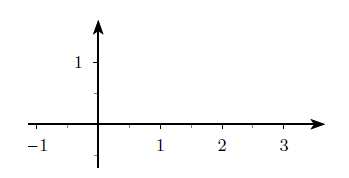
\includegraphics[scale=.8]{cours_methode1.eps}                                    \end{center}

\begin{enumerate}
\def\labelenumi{\arabic{enumi}.}
\itemsep1pt\parskip0pt\parsep0pt
\item
  Montrer que cette fonction est une fonction de densité de probabilité
  sur l'intervalle \([0;2]\).
\item
  Soit \(X\) est une variable aléatoire dont la loi de probabilité a
  pour densité \(f\). Calculer \(P(X\leqslant1,7)\).
\item
  Calculer l'espérance mathématique de \(X\).
\end{enumerate}

\end{methode}

\section{La loi uniforme}\label{la-loi-uniforme}

\begin{definition}{}
 
Étant donnés deux réels \(a\) et \(b\), avec \(a\leqslant b\), on
appelle \emph{loi uniforme} sur l'intervalle \([a;b]\) la loi dont la
fonction de densité est la fonction constante définie par :
\[\forall x\in [a;b], f(x)=\frac{1}{b-a}.\]

\end{definition}

\vspace{.5cm}

\begin{theoreme}{}
 
Si \(X\) est une variable aléatoire de loi uniforme sur un intervalle
\([a;b]\), alors son espérance mathématique est donnée par la formule
suivante : \[E(X)=\frac{b+a}{2}\]

\end{theoreme}

\begin{proof}
 voir cahier.
\end{proof}

%\vspace{.5cm}

\begin{remarque}
 
La commande \texttt{NbrAléat} de la calculatrice retourne une nombre
décimal choisi au hasard dans l'intervalle \([0;1]\), avec 10 décimales.
En assimilant ce choix au choix d'un nombre réel au hasard dans
l'intervalle \([0;1]\), on peut considérer que cette commande
\emph{simule} une loi uniforme sur l'intervalle \([0;1]\).

\end{remarque}

\vspace{.5cm}

\begin{methode}{Utilisation d'une loi uniforme}

Martin arrive tous les matins entre $7:15$ et $7:35$ à son arrêt de bus. On
considère que son heure d'arrivée est une variable aléatoire suivant une
loi uniforme, notée \(X\), sur l'intervalle \([15;35]\).

Le bus qu'il attend passe à $7:00$, puis toutes les 10 minutes.

\begin{enumerate}
\def\labelenumi{\arabic{enumi}.}
\itemsep1pt\parskip0pt\parsep0pt
\item
  Quelle est la probabilité que Martin attende moins de 5 min le
  prochain bus ?
\item
  S'il rate le bus de $7:30$, Martin arrive en retard. Quelle est la
  probabilité que Martin soit en retard ?
\end{enumerate}

\end{methode}

\section{La loi exponentielle}\label{la-loi-exponentielle}

Dans ce paragraphe, nous allons étudier un exemple un peu plus général
que ceux des paragraphes précédents. La loi exponentielle est en effet
une loi de probabilité à densité définie sur l'intervalle
$[0;+\infty[$, et non sur un intervalle du type
\([a;b]\).

Soit \(\lambda\) un réel strictement positif. On a alors, pour tout réel
\(t\) :
\(\int_0^t \lambda e^{-\lambda x} = [-e^{-\lambda x}]_0^t = 1-e^{-\lambda t}\).

On a donc :
\(\lim_{t\rightarrow +\infty}\int_0^t \lambda e^{-\lambda x} = 1\).

Par analogie avec les definitions du premier paragraphe, on peut donc
dire que la fonction \(f:x\mapsto \lambda e^{-\lambda x}\) est une
fonction de densité sur l'intervalle $[0;+\infty[$.

\vspace{.5cm}

\begin{definition}{}
 
Soit \(\lambda\) un réel strictement positif.

On appelle \emph{loi exponentielle} de paramètre \(\lambda\) la loi de
probabilité de densité \(f:x\mapsto \lambda e^{-\lambda x}\) , définie
sur $[0;+\infty[$.

\end{definition}

\vspace{.5cm}

\begin{theoreme}{}
 
Si \(X\) est une variable aléatoire de loi exponentielle de paramètre
\(\lambda>0\), alors l'espérance mathématique de \(X\) est donnée par :

\[E(X)=\lim_{t\rightarrow+\infty}\int_0^t x \times \lambda e^{-\lambda x} =\frac{1}{\lambda}\]

\end{theoreme}

\begin{proof}
 Voir cahier. Attention, cette démonstration est
exigible.
\end{proof}

\vspace{.5cm}

\begin{methode}{Utilisation d'une loi exponentielle (Pondichéry 2014)}

La durée de vie, exprimée en années, d'un moteur pour automatiser un
portail fabriqué par une entreprise A est une variable aléatoire \(X\)
qui suit une loi exponentielle de paramètre \(\lambda>0\).

\begin{enumerate}
\def\labelenumi{\arabic{enumi}.}
\itemsep1pt\parskip0pt\parsep0pt
\item
  On sait que \(P(X\leqslant 2)=0,15\). Déterminer la valeur exacte de
  \(\lambda\) (dans la suite de l'exercice on prendra 0,081 pour valeur
  de \(\lambda\)).
\item
  Calculer \(P(X\geqslant 3)\).
\item
  Calculer l'espérance de la variable aléatoire \(X\) et donner une
  interprétation de ce résultat.
\end{enumerate}

\end{methode}

\vspace{.5cm}

La loi exponentielle a une propriété bien particulière, dite de ``durée
de vie sans vieillissement''. Cette propriété traduit l'idée que, si la
variable aléatoire \(X\) modélise par exemple la durée de vie d'un
composant électronique, la probabilité que ce composant fonctionne
encore au moins 10 heures sachant qu'il a déjà fonctionné $n$ heures ne
dépend pas de \(n\) : elle est égale à la probabilité que ce composant
fonctionne au moins 10 heures quand il est neuf.

\vspace{.5cm}

\begin{theoreme}{durée de vie sans vieillissement}

Si \(X\) est une variable aléatoire de loi exponentielle de paramètre
\(\lambda>0\), alors pour tous réels positifs \(t\) et \(h\), on a :

\[P_{X\geqslant t}(X\geqslant t+h)=P(X\geqslant h)\]

\end{theoreme}

\begin{proof}
 Voir cahier. Cette preuve est au programme, non
exigible.
\end{proof}

\vspace{.5cm}

\begin{methode}{Utilisation d'une exponentielle - Suite - (Pondichéry
2014)}

La durée de vie, exprimée en années, d'un moteur pour automatiser un
portail fabriqué par une entreprise A est une variable aléatoire \(X\)
qui suit une loi exponentielle de paramètre \(\lambda>0\).

\begin{enumerate}
\def\labelenumi{\arabic{enumi}.}
\setcounter{enumi}{3}
\itemsep1pt\parskip0pt\parsep0pt
\item
  Le moteur a déjà fonctionné durant 3 ans. Quelle est la probabilité
  pour qu'il fonctionne encore 2 ans?
\end{enumerate}

\end{methode}

\end{document}
